\section{Analiza oprogramowania}
\subsection{Firmware}
Jako firmware określane jest oprogramowanie którego komendy są wykonywane przez
mikrokontroler. W tym podrozdziale zajmiemy się kodem źródłowym opisującym sposób
działania robota.

Pliki składające się na kod źródłowy robota możemy podzielić na dwa rodzaje:
\begin{itemize}
 \item napisane przez autora
 \item dostarczone przez producenta mikrokontrolera
\end{itemize}

Pliki dostarczone przez producenta mikrokontrolera są po prostu biblioteką,
dzięki której programista może kontrolować działanie różnych urządzeń
peryferyjnych mikrokontrolera. Biblioteka wykorzystana przez twórcę Dark
Explorera bazuje na prostych funkcjach wpisujących podawane wartości do
odpowiednich rejestrów mikrokontrolera. Można powiedzieć, że jest to biblioteka
niskopoziomowa. Wymaga ona dużej wiedzy na~temat urządzeń peryferyjnych z
których mamy zamiar korzystać oraz rejestrów które nimi sterują. Praktycznie
nie jest możliwe oprogramowanie robota przy pomocy tej~biblioteki bez
wcześniejszego dokładnego zaznajomienia się z notą katalogową mikrokontrolera
AT91Sam7S256. Podczas rozwoju robota przydatnym byłoby wykorzystanie innej
biblioteki, która jest bardziej przyjazna dla programisty.

Bazowa wersja firmware'u napisanego przez autora Dark Explorera została podzielona na sześć plików:
\begin{basedescript}{\desclabelstyle{\pushlabel}\desclabelwidth{40mm}}
\setlength{\parsep}{0pt}
\setlength{\itemsep}{0mm}
\setlength{\parskip}{0pt}
\item[board.h]
	Plik nagłówkowy z informacjami dotyczącymi mikromodułu mikrokontrolera
\item[pio.h] 
	Definicje określające wejścia i wyjścia ogólnego przeznaczenia zamontowane na~płycie głównej robota
\item[main.c] 
	Inicjalizacje początkowe, obsługa przerwań systemowych, interpretacja komend bluetooth, pętla główna programu
\item[peripherals.c] 
	Funkcje do obsługi urządzeń peryferyjnych
\item[rozpoznawanie.c] 
	Analiza i rozpoznawanie obrazu
\item[utils.c] 
	Procedury sterujące i obliczeniowe wyższego poziomu
\end{basedescript}

Biorąc pod uwagę ilość kodu znajdującą się w plikach, taki podział wydaje się być
wystarczający. W przyszłości trzeba zadbać o gęstsze partycjonowanie kodu
źródłowego na logiczne bloki w celu zapewnienia przejrzystości kodu źródłowego.

\subsection{Aplikacja zarządzająca}
Do kontrolowania robota została stworzona aplikacja graficzna (rys.
\ref{fig:AplikacjaZarz}) działająca pod systemem Windows. Interfejs graficzny
aplikacji jest atrakcyjny i przejrzysty. Pozwala ona na kontrolę następujących funkcji robota:
\begin{itemize}
\setlength{\parsep}{2pt}
\setlength{\itemsep}{2mm}
\setlength{\parskip}{4pt}
 \item kontrola kierunku i szybkości jazdy robota za pomocą wektora wodzącego oraz klawiatury
 \item kontrola wieży obserwacyjnej
 \item włączanie oraz wyłączanie diody oświetlającej
 \item informacja o stanie akumulatorów
 \item zarządzanie trybem autonomicznym robota
 \item konfiguracja oraz status połączenia bluetooth
\end{itemize}

\begin{figure}[!ht]
 \centering
 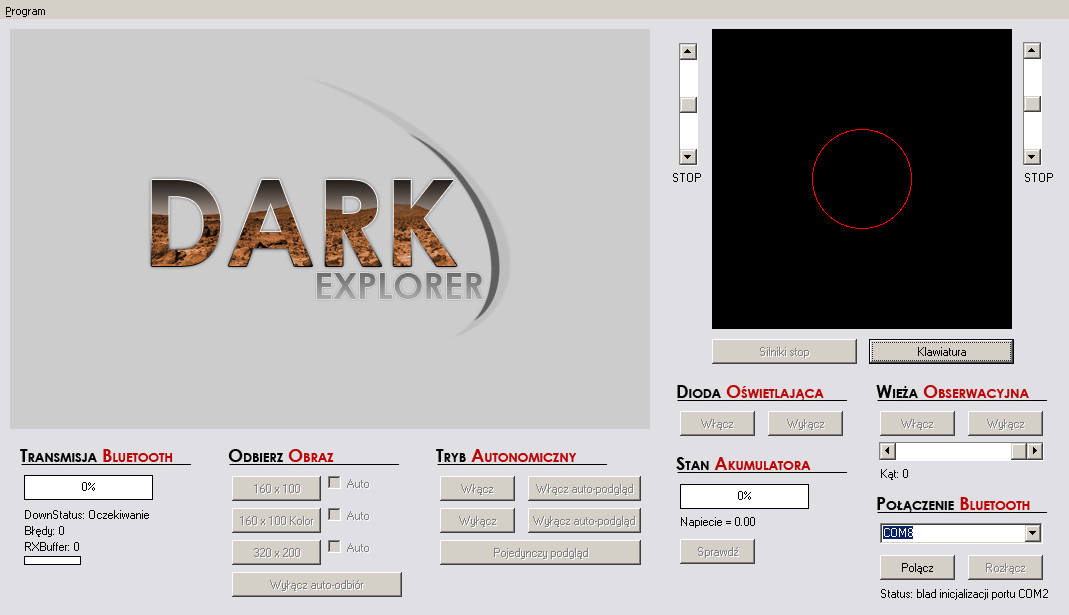
\includegraphics[width=\textwidth]{../images/ch02/decontrollprogram.png}
 \caption{Okno aplikacji zarządzającej Dark Explorera}
 \label{fig:AplikacjaZarz}
\end{figure}

Aplikacja zarządzająca została napisana tylko na jeden rodzaj systemu
operacyjnego. Nie ma możliwości kontrolowania robota przy pomocy komputera z
zainstalowanym systemem operacyjnym innym niż Microsoft Windows. Dlatego też,
konieczne będzie stworzenie aplikacji zarządzającej, którą będzie można
modyfikować oraz uruchomić na~dowolnym systemie.

W celu komunikacji z robotem, aplikacja zarządzająca wysyła do niego odpowiednie
komunikaty. Komunikaty te składają się z pojedynczego znaku i liczby. Możliwe, że
w przypadku obsługi większej ilości urządzeń na Dark Explorerze, będzie konieczne
stworzenie bardziej zaawansowanego protokołu komunikacyjnego. Zapewni to
możliwość sprawdzenia czy dana komenda jest poprawnie skonstruowana, czy może
zawiera jakieś błędy które pojawiły się podczas transmisji.

Zarówno w aplikacji zarządzającej jak i na robocie został zastosowany mechanizm
retransmisji pakietów z obrazem w przypadku błędów w trakcie połączenia. Jest to
bardzo dobry pomysł w szczególności w przypadku przesyłania takiej ilości danych
jaką generuje kamera.
